\chapter{Bài 9. Tổng hợp lực - Phân tích lực}
\begin{center}
	\textit{(3 tiết)}
\end{center}
\section{MỤC TIÊU DẠY HỌC}
\begin{center}
	\begin{longtable}{|M{2.5cm}|L{12.5cm}|M{2cm}|}
		\hline
		\thead{Biểu hiện\\ năng lực} & \thead{Mục tiêu} & \thead{STT}\\
		\hline
		\multicolumn{3}{|c|}{\textbf{ Năng lực vật lí}}\\
		\hline
		1.1 & Nêu được quy tắc tổng hợp phân tích lực.&1 \\
		\hline
		1.1 & Phát biểu được quy tắt hình bình hành.  &2\\
		\hline
		1.1 & Nêu được khái niệm về các lực cân bằng, không cân bằng. & 3\\
		\hline
		1.2 & Dùng hình vẽ, tổng hợp được các lực trên một mặt phẳng. &4\\
		\hline
		1.2 & Dùng hình vẽ, phân tích được một lực thành các lực thành phần vuông góc. & 5\\
		\hline
		1.2 & Mô tả được bằng ví dụ thực tế về lực bằng nhau, không bằng nhau.& 6\\
		\hline
		2.3 & Thảo luận để thiết kế phương án hoặc lựa chọn phương án và thực hiện phương án, tổng hợp được hai lực đồng quy và hai lực song song bằng dụng cụ thực hành.& 7\\
		\hline
		\multicolumn{3}{|c|}{\textbf{Năng lực chung}}\\
		\hline
		TC - TH& Tích cực thực hiện các nhiệm vụ thảo luận và thiết kế phương án thí nghiệm của nhóm, tích cực nghiên cứu SGK và tập hợp kiến thức của bản thân, suy luận để trả lời các câu hỏi của GV.	& 8 \\
		\hline
		GQVĐ - ST& Thảo luận và nêu được ý tưởng, phương án thí nghiệm phù hợp để tổng hợp được hai lực có giá đồng quy. &9\\
		\hline
	\end{longtable}
\end{center}
\section{THIẾT BỊ DẠY HỌC VÀ HỌC LIỆU}
\begin{itemize}
	\item Tivi/máy chiếu;
	\item Bộ dụng cụ thực hành tổng hợp lực đồng quy và tổng hợp lực song song cùng chiều;
	\item SGK.
\end{itemize}
\section{TIẾN TRÌNH DẠY HỌC}
\subsection{TIẾN TRÌNH}\newpage
\begin{center}
	\begin{longtable}{|L{2.75cm}|C{1.25cm}|L{5cm}|L{3.5cm}|L{4cm}|}
		\hline
		\thead{Tiến trình} & \thead{Mục\\tiêu} & \thead{Nội dung dạy học \\trọng tâm} & \thead{PP,\\ KTDH} & \thead{Phương pháp \\đánh giá}\\
		\hline
		\textbf{Hoạt động 1:} Hình thành khái niệm tổng hợp lực & 1, 8 & Khái niệm tổng hợp lực  & PPDH: Đàm thoại\newline KTDH: Chia sẻ nhóm đôi & GV đánh giá dựa trên câu trả lời của HS.\newline
		PP đánh giá: quan sát, nghe.  \\
		\hline
		\textbf{Hoạt động 2:} Tìm hiểu phương pháp tổng hợp lực trên một mặt phẳng & 2, 4, 8 & Phương pháp hình bình hành để cộng vector (mở rộng thêm phương pháp tam giác vector và đa giác vector) & PPDH: Dạy học hợp tác & GV đánh giá dựa trên câu trả lời của HS.\newline
		PP đánh giá: quan sát, nghe.  \\
		\hline
		\textbf{Hoạt động 3:} Vận dụng phương pháp tổng hợp lực trên một mặt phẳng & 2, 4, 8 & Phương pháp hình bình hành/tam giác vector để tìm hợp lực của hai lực đồng quy & PPDH: Đàm thoại \newline KTDH: Tia chớp& GV đánh giá dựa trên bài tập ví dụ của HS.\newline
		PP đánh giá: quan sát, nghe.  \\
		\hline
		\textbf{Hoạt động 4:} Hình thành khái niệm về các lực cân bằng và không cân bằng & 3, 6 & Điều kiện cân bằng của chất điểm & PPDH: Đàm thoại & GV đánh giá dựa trên câu trả lời của HS.\newline
		PP đánh giá: quan sát, nghe.  \\
		\hline
		\textbf{Hoạt động 5:} Tìm hiểu phương pháp phân tích một lực thành các lực thành phần vuông góc & 5, 8 & Phân tích một lực thành 2 lực thành phần vuông góc & PPDH: Đàm thoại\newline
		KTDH: Tia chớp & GV đánh giá dựa trên câu trả lời của HS.\newline
		PP đánh giá: quan sát, nghe.  \\
		\hline
		\textbf{Hoạt động 6:} Tìm hiểu phương pháp tổng hợp lực song song cùng chiều & 7, 9 & Quy tắc tổng hợp lực song song cùng chiều  & PPDH: Dạy học hợp tác& GV đánh giá dựa trên báo cáo thí nghiệm của nhóm học sinh.\newline
		PP đánh giá: quan sát, nghe.  \\
		\hline
		\textbf{Hoạt động 7:} Vận dụng phương pháp tổng hợp hai lực song song cùng chiều & 7, 8& Tổng hợp hai lực song song cùng chiều & PPDH: Đàm thoại \newline KTDH: Tia chớp& GV đánh giá dựa trên bài tập ví dụ của HS.\newline
		PP đánh giá: quan sát, nghe.  \\
		\hline
		\textbf{Hoạt động 8:} Luyện tập	& 1, 2, 3, 4, 5, 6, 8  & Luyện tập bài tập tổng hợp lực đồng quy, tổng hợp lực song song cùng chiều. & PPDH:  Đàm thoại& GV đánh giá dựa trên bài tập cá nhân của học sinh.\newline
		PP đánh giá: quan sát, nghe. \\
		\hline
	\end{longtable}
\end{center}
\subsection{CÁC HOẠT ĐỘNG HỌC}
% ==========================================================================================
\hoatdong
{Hình thành khái niệm tổng hợp lực.
}
{HS nêu được khái niệm tổng hợp lực và quy tắc tổng hợp lực.
}
{Kết quả trả lời của HS cho các câu hỏi gợi mở của GV.
}
{\textit{\underline{* GV chuyển giao nhiệm vụ học tập}}
	\begin{itemize}[label=-]
		\item GV yêu cầu HS thảo luận nhóm đôi và cho biết trong mỗi trường hợp dưới đây vật sẽ di chuyển theo hướng nào? HS cần đưa ra lời giải thích cho mỗi nhận định.
		\begin{center}
			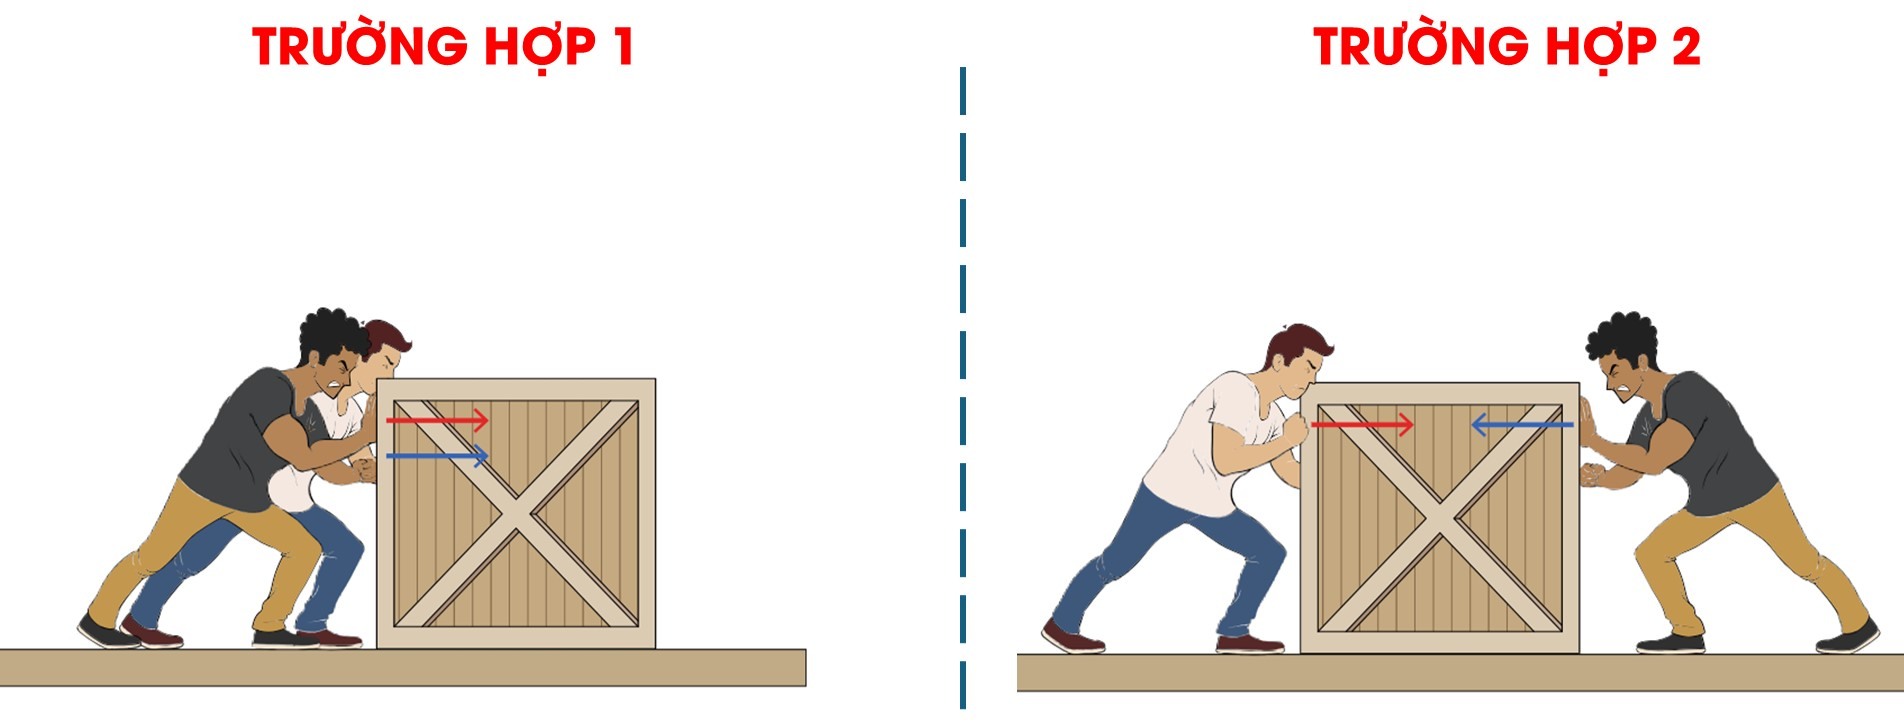
\includegraphics[scale=0.4]{figs/G10-BAI9-1}
		\end{center}
		\begin{center}
			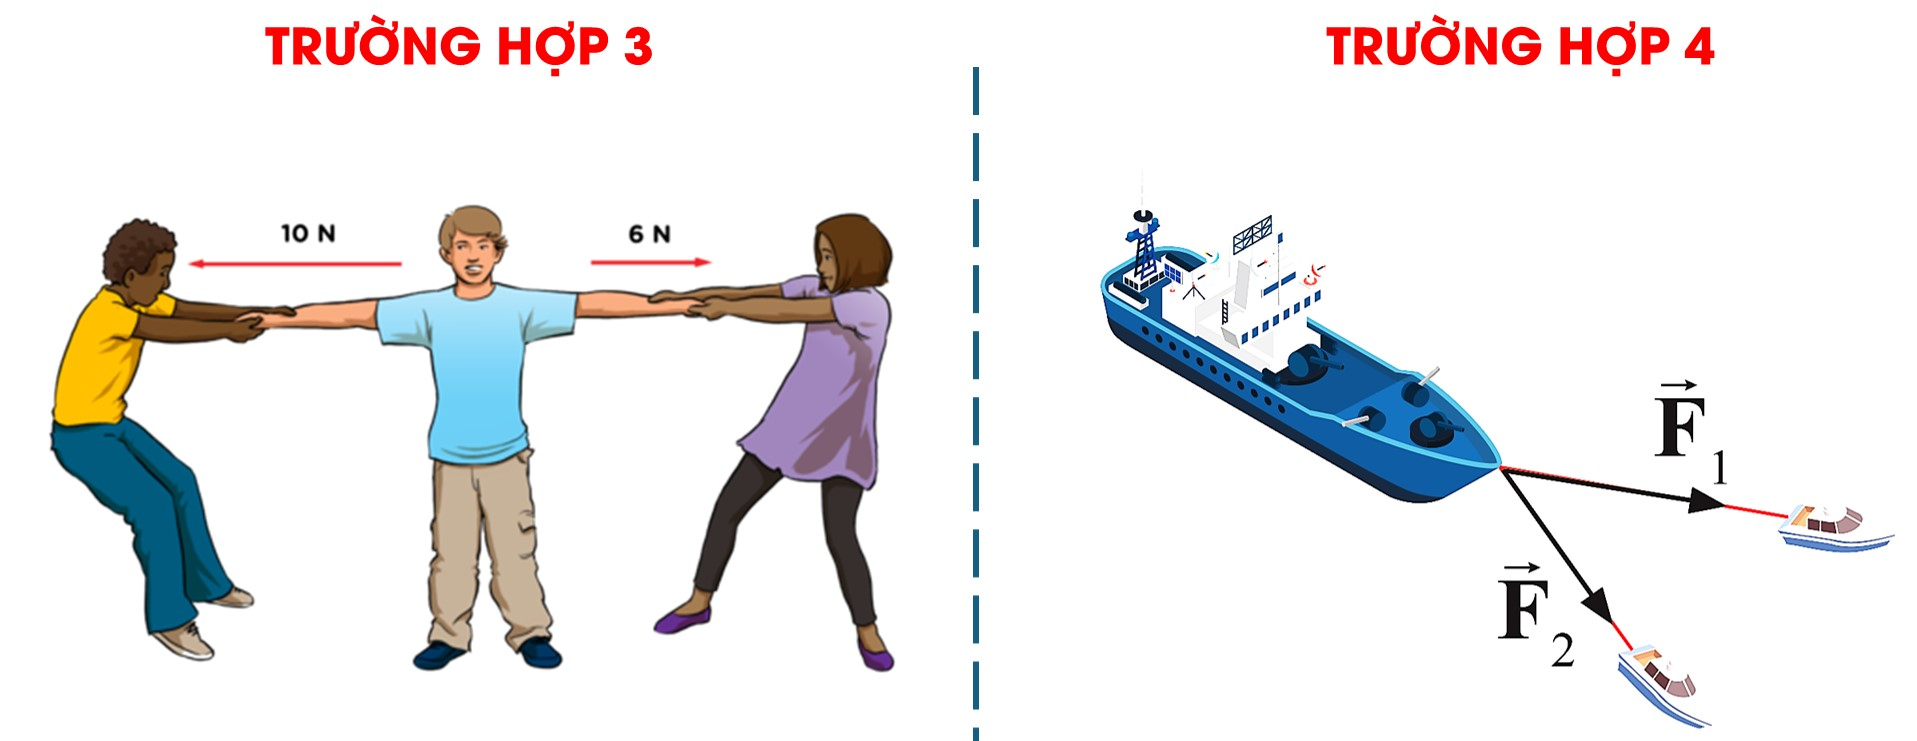
\includegraphics[scale=0.4]{figs/G10-BAI9-2}
		\end{center}
		\item Từ câu trả lời của HS, GV dẫn dắt đến khái niệm tổng hợp lực.
		\item GV giới thiệu: Về mặt toán học, ta có thể tìm hợp lực bằng phép cộng vector: $$\vec{F}=\vec{F}_1+\vec{F}_2+\vec{F}_3+\dots$$
	\end{itemize}
		\textit{\underline{* HS thực hiện nhiệm vụ học tập}}\\
	HS chú ý lắng nghe và tích cực trả lời các câu hỏi gợi ý của GV.\\
	\textit{\underline{* HS báo cáo kết quả nhiệm vụ học tập}}\\
	GV lần lượt mời HS trả lời câu hỏi.
}
% ==========================================================================================
\hoatdong
{Tìm hiểu phương pháp tổng hợp lực trên một mặt phẳng.
}
{\begin{itemize}
		\item HS sử dụng được phương pháp hình bình hành để tìm hợp lực.
		\item HS dựng được tam giác vector/đa giác vector để tìm hợp lực.
	\end{itemize}
}
{Kết quả trả lời của HS cho các câu hỏi gợi mở của GV và bài tập ví dụ.
}
{\textit{\underline{* GV chuyển giao nhiệm vụ học tập}}
	\begin{itemize}[label=-]
		\item GV ôn lại cho HS quy tắc hình bình hành để cộng vector (HS đã học trong chương trình môn Toán).
		\begin{center}
			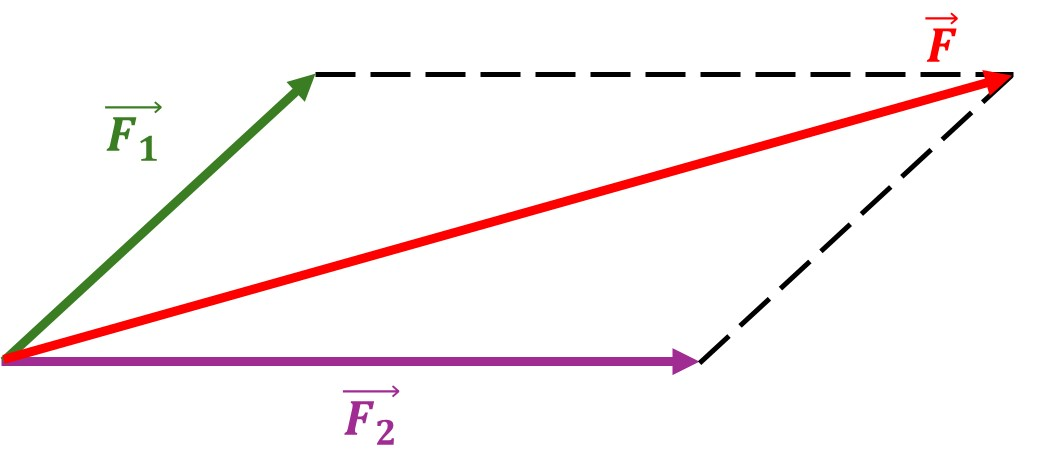
\includegraphics[scale=0.5]{figs/G10-BAI9-3}
		\end{center}
		\item GV giới thiệu cho HS phương pháp tam giác vector.
		\item GV yêu cầu HS dựa vào phương pháp tam giác vector tìm độ lớn hợp lực trong các trường hợp đặc biệt: $\vec{F}_1\uparrow\uparrow\vec{F}_2$; $\vec{F}_1\uparrow\downarrow \vec{F}_2$; $\vec{F}_1\bot\vec{F}_2$.
		\begin{center}
			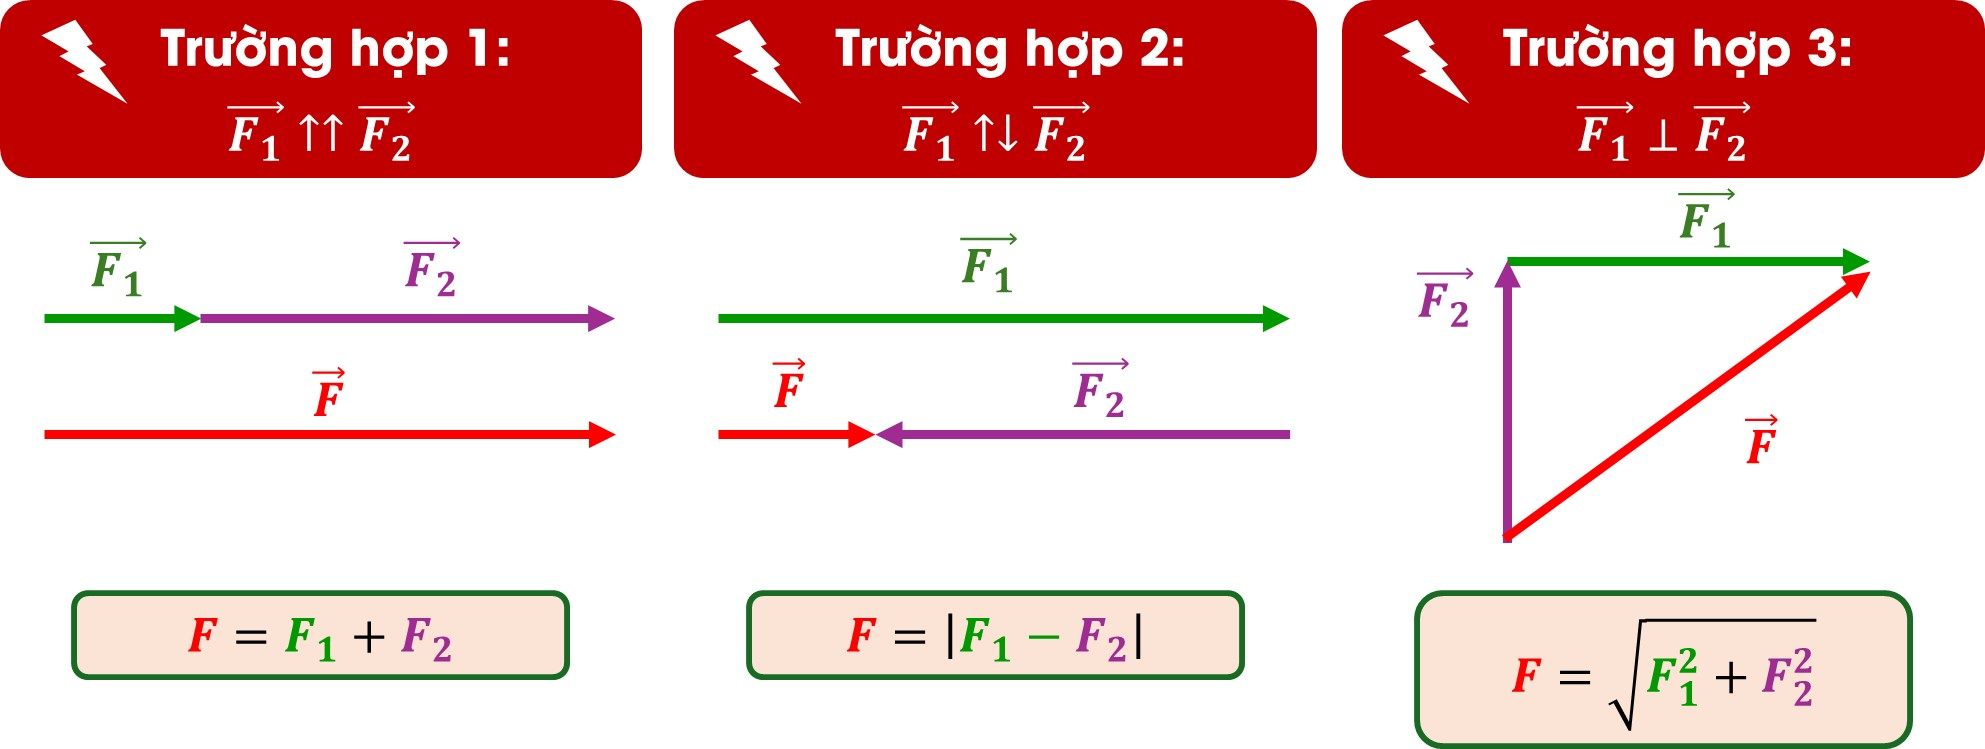
\includegraphics[scale=0.5]{figs/G10-BAI9-4}
		\end{center}
		\item GV dùng bộ thí nghiệm gắn bản thực hiện thí nghiệm minh họa phương pháp tổng hợp lực đồng quy.
		\begin{center}
			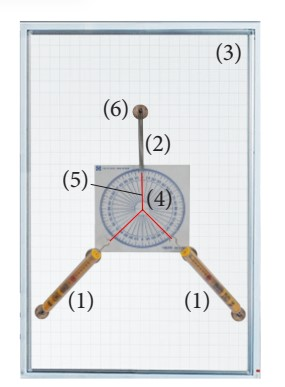
\includegraphics[scale=1]{figs/G10-BAI9-5}
		\end{center}
		\textbf{Dụng cụ:}
		\begin{itemize}[label=$\bullet$]
			\item 3 lực kế (1) có giới hạn đo $\SI{5}{\newton}$, lò xo (2) có độ cứng phù hợp;
			\item bảng từ (3);
			\item thước eke ba chiều, thước đo góc (4) gắn trên bảng từ;
			\item dây nối ban nhánh (5) nhẹ, không dãn;
			\item nam châm (6).
		\end{itemize}
	\end{itemize}
	GV chia lớp học thành 6 nhóm.\\
	Dựa vào số đo góc $\alpha$ và độ lớn $\vec{F}_1$, $\vec{F}_2$, $\vec{F}_3$. GV yêu cầu các nhóm HS biểu diễn $\vec{F}_1$; $\vec{F}_2$, $\vec{F}_3$ theo tỉ xích xác định và chứng minh lực tổng hợp $\vec{F}$ nằm trên đường chéo hình bình hành với 2 cạnh là 2 lực thành phần.\\
	\textit{\underline{* HS thực hiện nhiệm vụ học tập}}
	\begin{itemize}[label=-]
		\item HS chú ý lắng nghe và tích cực trả lời các câu hỏi gợi ý của GV.
		\item HS hoạt động theo nhóm được GV phân công và hoàn thành nhiệm vụ chứng minh lực tổng hợp $\vec{F}$ nằm trên đường chéo hình bình hành với 2 cạnh là 2 lực thành phần.
	\end{itemize}
	\textit{\underline{* HS báo cáo kết quả nhiệm vụ học tập}}\\
	GV mời đại diện 1 nhóm HS lên trình bày kết quả thảo luận, 1 nhóm nhận xét kết quả nhóm trước đã trình bày.\\
	GV chỉnh lý, hợp thức hóa kiến thức.
}
% ==========================================================================================
\hoatdong
{Vận dụng phương pháp tổng hợp lực trên một mặt phẳng.
}
{HS vận dụng được quy tắc hình bình hành/tam giác vector để tìm hợp lực của hai lực đồng quy.
}
{Bài tập ví dụ của HS.
}
{\textit{\underline{* GV chuyển giao nhiệm vụ học tập}}\\
	GV sử dụng kĩ thuật tia chớp yêu cầu HS thực hiện Ví dụ 1.\\
	\textit{\underline{* HS thực hiện nhiệm vụ học tập}}\\
	HS thực hiện bài tập ví dụ theo hình thức cá nhân.\\
	\textit{\underline{* HS báo cáo kết quả nhiệm vụ học tập}}\\
	GV mời HS có kết quả nhanh nhất lên bảng trình bày bài tập ví dụ.\\
	Các HS còn lại theo dõi, nhận xét/đặt câu hỏi.\\
	GV chỉnh lí, hợp thức hóa kiến thức.
}
% ==========================================================================================
\hoatdong
{Hình thành khái niệm về các lực cân bằng và không cân bằng.
}
{HS nêu được khái niệm lực cân bằng và lực không cân bằng.
}
{Câu trả lời của HS.
}
{\textit{\underline{* GV chuyển giao nhiệm vụ học tập}}
	\begin{itemize}[label=-]
		\item GV yêu cầu HS nhận xét trạng thái chuyển động của thùng hàng và sợi dây trong 2 tình huống bên dưới.
		\begin{center}
			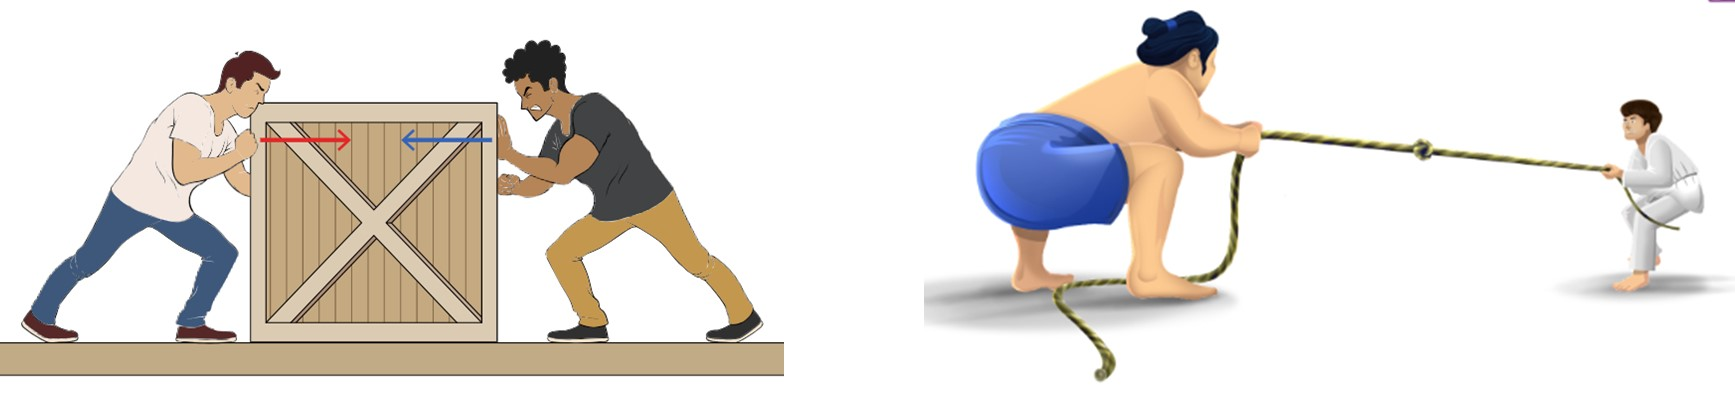
\includegraphics[scale=0.5]{figs/G10-BAI9-6}
		\end{center}
		\item Từ câu trả lời của HS, GV yêu cầu HS phát biểu điều kiện để chất điểm ở trạng thái cân bằng (đứng yên hoặc chuyển động thẳng đều).
		\item GV tổng hợp lại khái niệm 2 lực cân bằng và 2 lực không cân bằng từ các câu trả lời của HS.
	\end{itemize}
	\textit{\underline{* HS thực hiện nhiệm vụ học tập}}\\
	HS chú ý lắng nghe và tích cực trả lời các câu hỏi gợi ý của GV.\\
	\textit{\underline{* HS báo cáo kết quả nhiệm vụ học tập}}\\
	GV lần lượt mời HS trả lời câu hỏi.
}
% ==========================================================================================
\hoatdong
{Tìm hiểu phương pháp phân tích một lực thành các lực thành phần vuông góc.
}
{HS phân tích được một lực thành 2 lực thành phần vuông góc.
}
{Câu trả lời và bài tập ví dụ của HS.
}
{\textit{\underline{* GV chuyển giao nhiệm vụ học tập}}
	\begin{itemize}[label=-]
		\item GV giới thiệu lại cho HS phương pháp tìm độ lớn hình chiếu trên các trục $Ox$, $Oy$.
		\begin{center}
			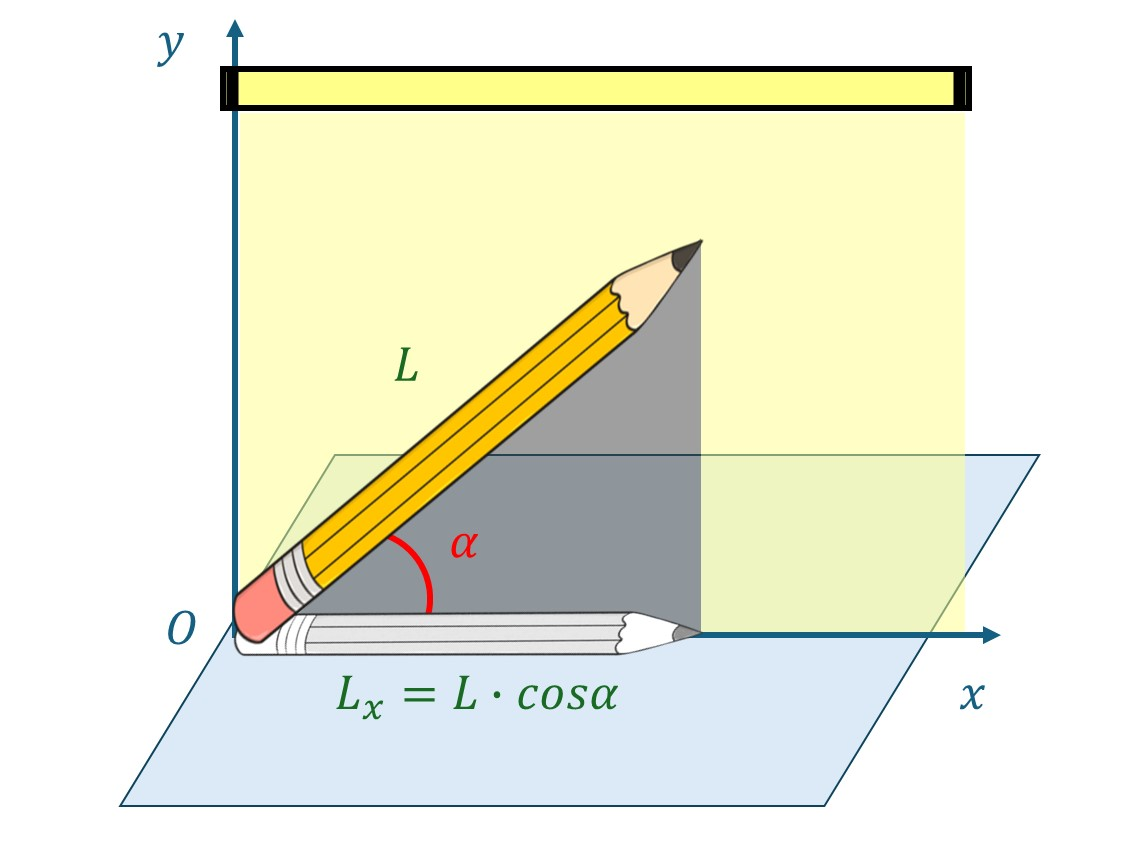
\includegraphics[scale=0.5]{figs/G10-BAI9-7}
		\end{center}
		\begin{center}
			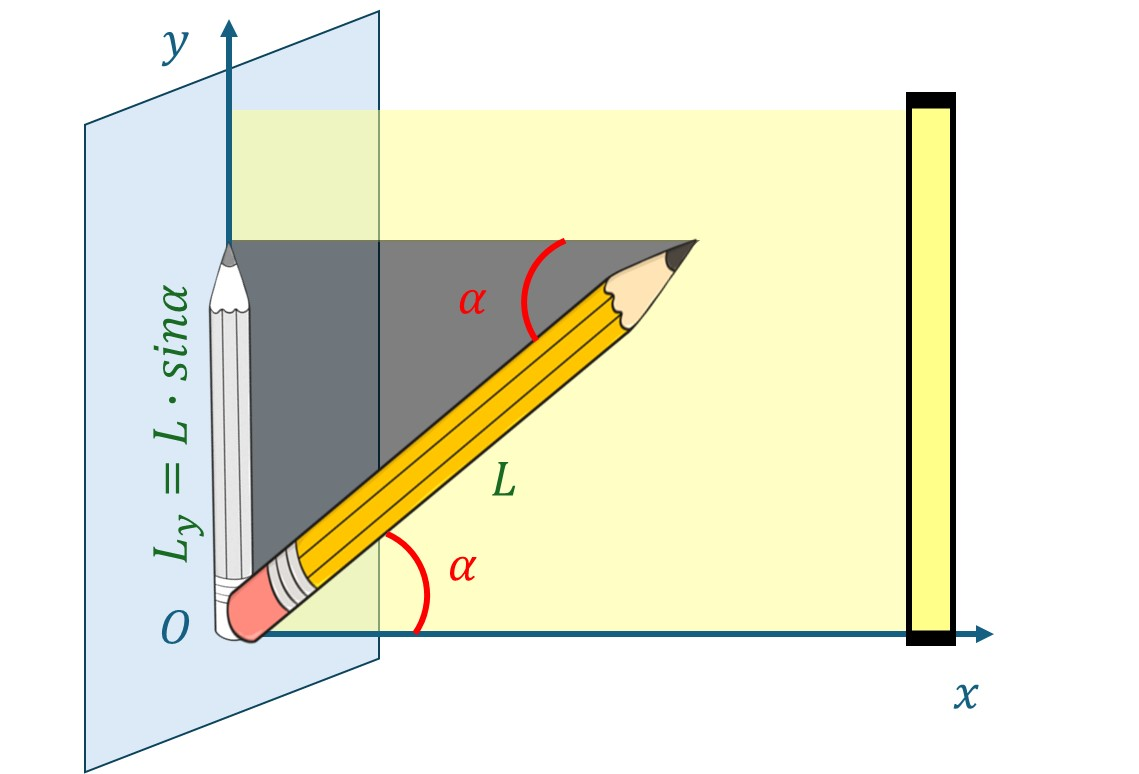
\includegraphics[scale=0.5]{figs/G10-BAI9-8}
		\end{center}
		\item GV yêu cầu HS phân tích lực $\vec{F}$ thành 2 thành phần $\vec{F}_x$ và $\vec{F}_y$.
		\begin{center}
			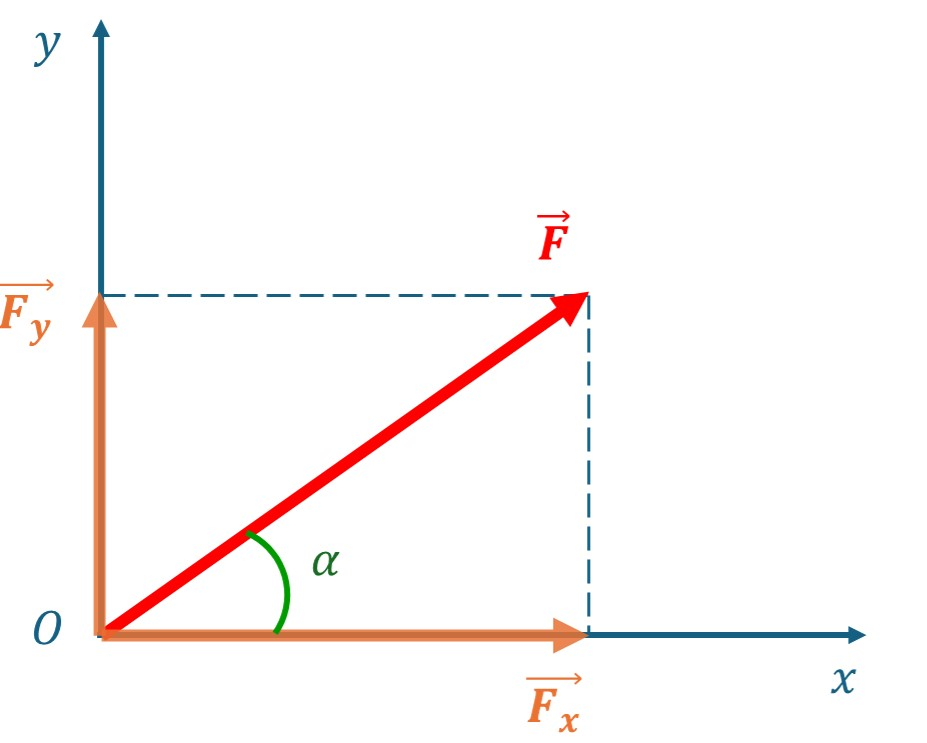
\includegraphics[scale=0.5]{figs/G10-BAI9-9}
		\end{center}
		\item GV yêu cầu HS thực hiện Ví dụ 2, Ví dụ 3, Ví dụ 4.
	\end{itemize}
	\textit{\underline{* HS thực hiện nhiệm vụ học tập}}\\
	HS chú ý lắng nghe và tích cực trả lời các câu hỏi gợi ý của GV.\\
	HS thực hiện Ví dụ 2 và Ví dụ 3.\\
	\textit{\underline{* HS báo cáo kết quả nhiệm vụ học tập}}\\
	GV lần lượt mời HS trả lời câu hỏi và lên bảng giải bài tập Ví dụ.
}
% ==========================================================================================
\hoatdong
{Tìm hiểu phương pháp tổng hợp lực song song cùng chiều.
}
{HS xác định được hợp lực của hai lực song song cùng chiều.
}
{Báo cáo thí nghiệm tổng hợp lực song song cùng chiều của HS.
}
{\textit{\underline{* GV chuyển giao nhiệm vụ học tập}}\\
	\begin{itemize}[label=-]
		\item GV chia lớp thành 6 nhóm.
		\item GV giới thiệu bộ dụng cụ thí nghiệm tổng hợp lực song song cùng chiều.
		\begin{center}
			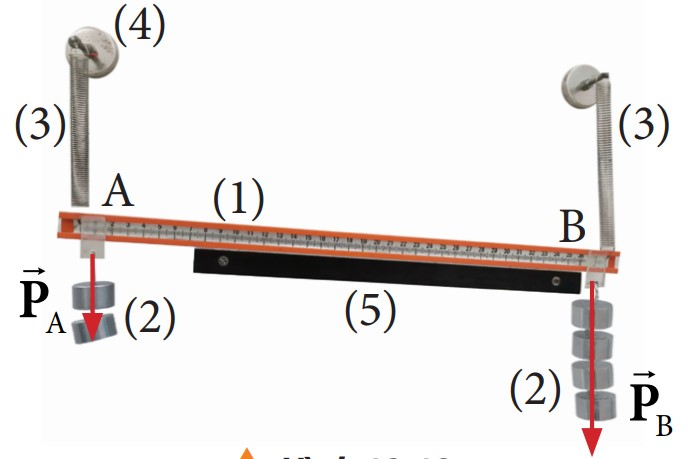
\includegraphics[scale=0.7]{figs/G10-BAI9-10}
		\end{center}
		\textbf{Dụng cụ:}\\
		\begin{itemize}[label=$\bullet$]
			\item Thước nhôm nhẹ (1) có độ chia đến $\si{\milli\meter}$, có móc treo di chuyển được;
			\item các quả cân (2) có khối lượng $\SI{50}{\gram}$;
			\item hai lò xo (3);
			\item bảng từ, nam châm (4);
			\item thước định vị (5).
		\end{itemize}
		\item GV hướng dẫn HS các bước tiến hành thí nghiệm:
		\begin{enumerate}[label=\bfseries $\bullet$ Bước \arabic*:, leftmargin=2cm]
			\item Bố trí thí nghiệm theo gợi ý: gắn hai đầu thước nhôm nhẹ với hai lò xo và treo lên bảng từ bằng hai nam châm.
			\item Treo vào hai điểm A, B ở hai đầu của thước nhôm một số quả cân (khối lượng mỗi bên khác nhau). Đánh dấu vị trí cân bằng mới này của thước nhờ vào eke ba chiều. Ghi giá trị trọng lượng $P_{\mathrm{A}}$, $P_{\mathrm{B}}$ của các quả cân bên theo mẫu bảng bên dưới.
			\item Treo các quả cân vào cùng một vị trí trên thước AB sao cho thước trở lại đúng vị trí đánh dấu lúc đầu. Đo các giá trị OA và OB trên thước ghi theo mẫu bảng bên dưới.
			\begin{center}
				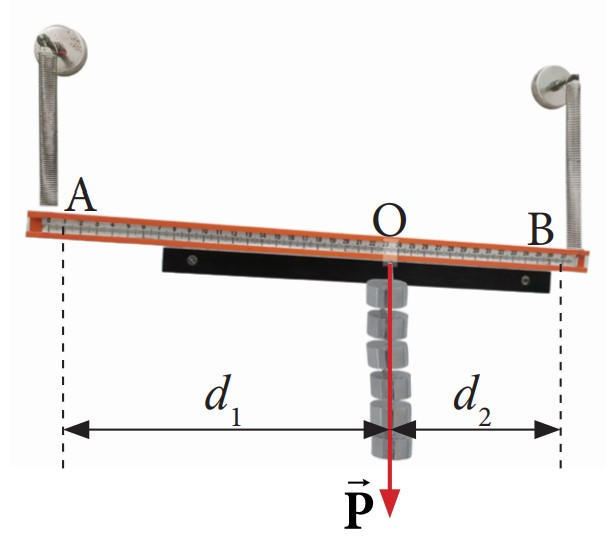
\includegraphics[scale=0.7]{figs/G10-BAI9-11}
			\end{center}
		\end{enumerate}
		\begin{center}
			\textbf{Bảng số liệu thực nghiệm tổng hợp hai lực song song}\\
			Chọn $P_{\mathrm{A}}=\dots\ \si{\newton}$, $P_{\mathrm{B}}=\dots\ \si{\newton}$\\
			\begin{tabular}{|M{3cm}|M{2cm}|M{2cm}|M{2cm}|M{3cm}|}
				\hline
				\thead{Lần} & \thead{1} & \thead{2} &\thead{3} &\thead{Trung bình}\\
				\hline
				$\xsi{\mathrm{OA}}{\left(\si{\centi\meter}\right)}$& &&&\\
				\hline
					$\xsi{\mathrm{OB}}{\left(\si{\centi\meter}\right)}$& &&&\\
				\hline
			\end{tabular}
		\end{center}
		\item GV theo dõi, hỗ trợ HS trong quá trình các nhóm thực hiện thí nghiệm.
		\item GV yêu cầu các nhóm HS so sánh tỉ số $\dfrac{P_{\mathrm{A}}}{P_{\mathrm{B}}}$ và $\dfrac{\mathrm{OB}}{\mathrm{OA}}$.
	\end{itemize}
		\textit{\underline{* HS thực hiện nhiệm vụ học tập}}\\
	HS chú ý lắng nghe.\\
	HS hoạt động theo nhóm để thực hiện thí nghiệm tổng hợp lực song song cùng chiều.\\
		\textit{\underline{* HS báo cáo kết quả nhiệm vụ học tập}}\\
	Các nhóm nộp lại báo cáo thí nghiệm cho GV.\\
	GV mời đại diện 1 nhóm HS báo cáo kết quả hoạt động. Các HS còn lại theo dõi, nhận xét.\\
	GV chỉnh lí, hợp thức hóa kiến thức.
}
% ==========================================================================================
\hoatdong
{Vận dụng phương pháp tổng hợp hai lực song song cùng chiều.
}
{HS vận dụng được quy tắc tổng hợp hai lực song song cùng chiều
}
{Bài tập ví dụ của HS.
}
{\textit{\underline{* GV chuyển giao nhiệm vụ học tập}}\\
	GV sử dụng kĩ thuật tia chớp yêu cầu HS thực hiện Ví dụ 5.\\
	\textit{\underline{* HS thực hiện nhiệm vụ học tập}}\\
	HS thực hiện bài tập ví dụ theo hình thức cá nhân.\\
	\textit{\underline{* HS báo cáo kết quả nhiệm vụ học tập}}\\
	GV mời HS có kết quả nhanh nhất lên bảng trình bày bài tập ví dụ.\\
	Các HS còn lại theo dõi, nhận xét/đặt câu hỏi.\\
	GV chỉnh lí, hợp thức hóa kiến thức.
}
\hoatdong{
	Luyện tập.
}
{
	HS xác định được hợp lực của hai lực đồng quy.\\
	HS xác định được hợp lực của hai lực song song cùng chiều.
}
{
	Bài tập cá nhân của học sinh.
}
{
	\textit{\underline{* GV chuyển giao nhiệm vụ học tập}}\\
	GV lần lượt chuyển giao từng bài tập, yêu cầu HS hoạt động cá nhân để giải.\\
	\textit{\underline{* HS thực hiện nhiệm vụ học tập}}\\
	HS \textit{(làm việc cá nhân)}:  Giải bài tập trong phiếu bài tập được GV giao. 
	
	GV: Theo dõi để phát hiện các HS gặp khó khăn, từ đó đưa ra sự định hướng, hỗ trợ phù hợp cho mỗi HS.\\
	\textit{\underline{* HS báo cáo kết quả thực hiện nhiệm vụ học tập}}\\
	GV: Mời HS lên bảng giải bài tập.
	
	HS: Đặt câu hỏi, góp ý.
	
	GV: Chỉnh lí, hợp thức hoá kiến thức.
}
\section{HỒ SƠ DẠY HỌC}
\subsection{NỘI DUNG DẠY HỌC}
\begin{enumerate}[label=\bfseries\Roman*.]
	\item \textbf{Tổng hợp lực - Phân tích lực}
	\begin{enumerate}[label=\bfseries\arabic*., leftmargin=1cm]
		\item \textbf{Tổng hợp lực} là thay thế các lực tác dụng đồng thời vào cùng một vật bằng một lực có tác dụng giống hệt như các lực ấy. Lực thay thế này gọi là hợp lực.\\
		\immini{\textbf{Quy tắc hình bình hành:} nếu hai lực đồng quy làm thành hai cạnh của một hình bình hành, thì đường chéo kẻ từ điểm đồng quy biểu diễn hợp lực của chúng $\vec{F}=\vec{F}_1+\vec{F}_2$.}
		{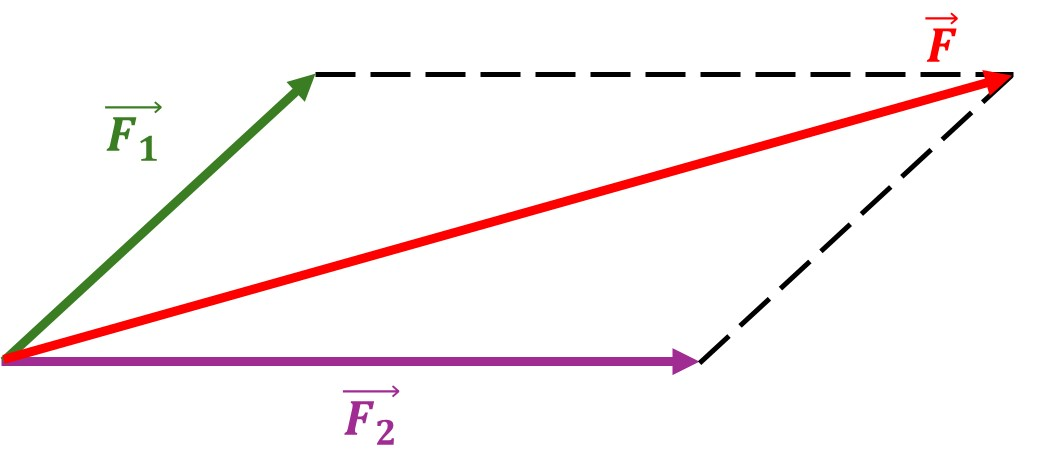
\includegraphics[scale=0.4]{figs/G10-BAI9-12}}
		\textbf{* Các trường hợp đặc biệt:}
		\begin{itemize}[label=$\bullet$]
			\item Nếu hai lực cùng chiều: $F=F_1+F_2$.
			\begin{center}
				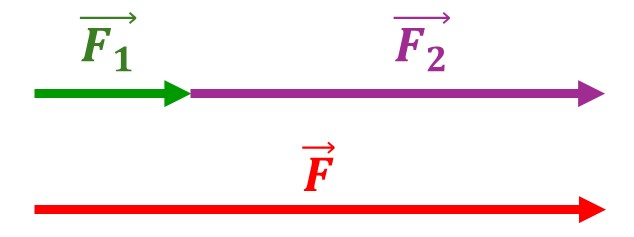
\includegraphics[scale=0.4]{figs/G10-BAI9-13}
			\end{center}
			\item Nếu hai lực ngược chiều: $F=\left|F_1-F-2\right|$.
			\begin{center}
				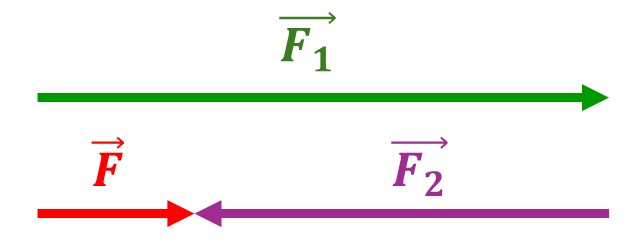
\includegraphics[scale=0.4]{figs/G10-BAI9-14}
			\end{center}
			\item Nếu hai lực vuông góc với nhau: $F=\sqrt{F^2_1+F^2_2}$.
			\begin{center}
				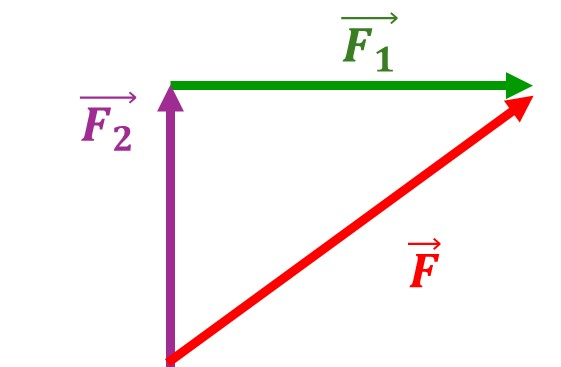
\includegraphics[scale=0.4]{figs/G10-BAI9-15}
			\end{center}
		\end{itemize}
		\item \textbf{Phân tích lực} là thay thế một lực bằng hai hay nhiều lực có tác dụng giống hệt như lực đó. Các lực thay thế này gọi là các lực thành phần.\\
		Phân tích lực cũng tuân theo quy tắc hình bình hành.
	\end{enumerate}
	\item \textbf{Quy tắc hợp hai lực song song cùng chiều}
		\begin{center}
		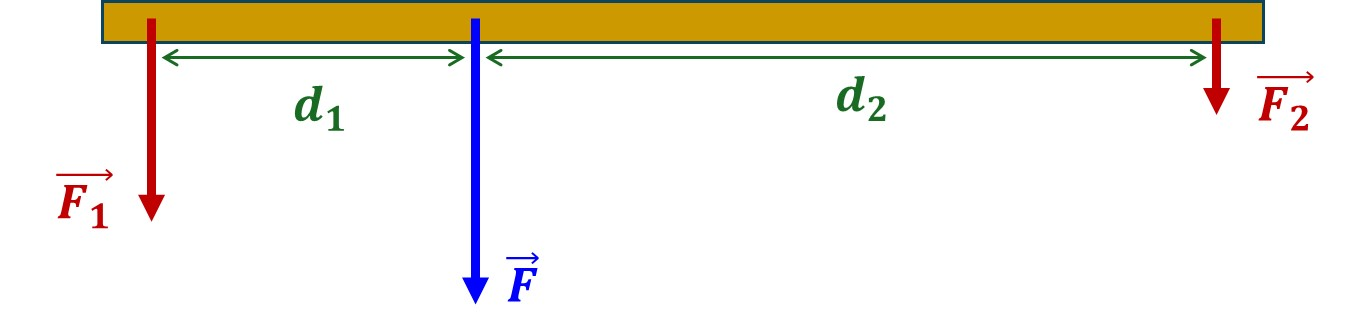
\includegraphics[scale=0.5]{figs/G10-BAI9-16}
	\end{center}
	\begin{itemize}[label=$\bullet$]
		\item Hợp lực của hai lực $\vec{F}_1$ và $\vec{F}_2$ song song, cùng chiều, tác dụng vào một vật rắn là một lực $\vec{F}$ song song, cùng chiều với hai lực và có độ lớn bằng tổng độ lớn hai lực đó.
		$$F=F_1+F_2.$$
		\item Giá của hợp lực $\vec{F}$ nằm trong mặt phẳng của $\vec{F}_1$, $\vec{F}_2$ và chia khoảng cách giữa hai lực này thành những đoạn tỉ lệ nghịch với độ lớn của hai lực:
		$$\dfrac{F_1}{F_2}=\dfrac{d_2}{d_1}.$$
	\end{itemize}
\end{enumerate}
\subsection{CÁC VÍ DỤ MINH HỌA}
\setcounter{ex}{0}
% ======================================================================
\begin{ex}
Hai lực có độ lớn $F_1=\SI{6}{\newton}$ và $F_2=\SI{8}{\newton}$ tác dụng đồng thời lên chất điểm. Tìm hợp lực của hai lực trên trong các trường hợp:
\begin{enumerate}[label=\alph*)]
	\item hai lực cùng hướng.
	\item hai lực ngược hướng.
	\item hai lực vuông phương.
\end{enumerate}
	\loigiai{}
\end{ex}
% ======================================================================
\begin{ex}
	\immini{Một cậu bé đang kéo thùng hàng trên mặt đất bằng sợi dây hợp với phương ngang góc $\SI{30}{\degree}$. Hãy tìm độ lớn lực kéo thành phần trên hai phương vuông góc và song song với mặt đất, biết độ lớn lực kéo của cậu bé tác dụng lên dây là \SI{12}{\newton}.
	}{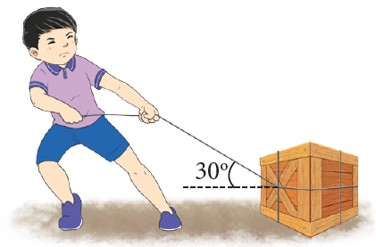
\includegraphics[scale=0.4]{figs/G10-BAI9-17}}
	\loigiai{}
\end{ex}
% ======================================================================
\begin{ex}
	\immini{Vật nặng trọng lượng \SI{20}{\newton} được đặt trên mặt phẳng nghiêng góc \SI{60}{\degree} như hình bên dưới. Xác định thành phần trọng lực tác dụng trên phương $Ox$, $Oy$ tương ứng. }
	{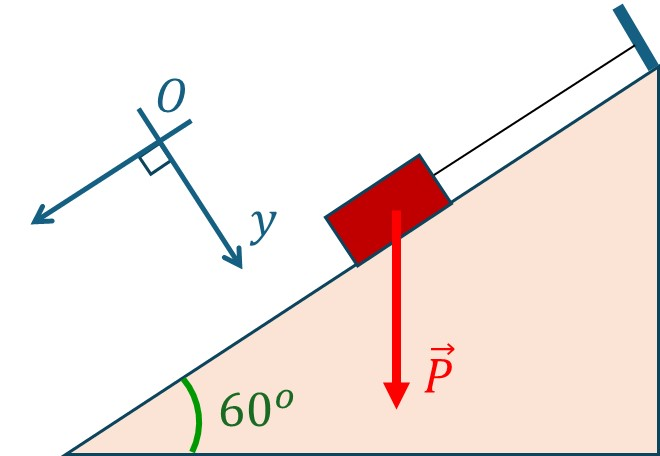
\includegraphics[scale=0.5]{figs/G10-BAI9-18}}
	\loigiai{}
\end{ex}
% ======================================================================
\begin{ex}
	\immini{Một cậu bé đang kéo thùng hàng trên mặt đất bằng sợi dây hợp với phương ngang góc \SI{30}{\degree}. Độ lớn lực ma sát trượt giữa thùng hàng và nền nhà là \SI{21.65}{\newton}. Cậu bé phải kéo thùng hàng với lực kéo bao nhiêu để thùng hàng chuyển động thẳng đều?}
	{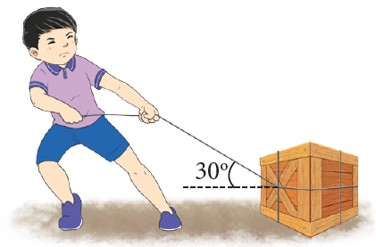
\includegraphics[scale=0.4]{figs/G10-BAI9-17}}
	\loigiai{}
\end{ex}
% ======================================================================
\begin{ex}
	\immini{Một người đang gánh lúa như hình bên dưới. Hỏi vai người đặt ở vị trí nào trên đòn gánh để đòn gánh có thể nằm ngang cân bằng trong quá trình di chuyển? Biết trọng lượng hai bó lúa lần lượt là \SI{70}{\newton} và \SI{50}{\newton}, chiều dài đòn gánh là \SI{1.5}{\meter}. Xem như điểm treo hai bó lúa sát hai đầu đòn gánh và bỏ qua trọng lượng đòn gánh.
	}{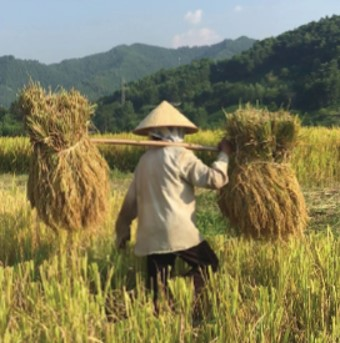
\includegraphics[scale=0.5]{figs/G10-BAI9-19}}
	\loigiai{}
\end{ex}